% Modelo GIQ para dissertações do PPGETI/UFC.
% Código de configuração MIT; textos demonstrativos originais CC0.
\documentclass[12pt,a4paper,oneside,openany,english,brazil,chapter=TITLE,sumario=abnt-6027-2012]{giq}
% SPDX-License-Identifier: MIT
% Configurações editáveis. Requer abntex2, biblatex-abnt e Biber instalados.
% Mude para \DocumentoInglestrue se redigir em ingles.
\newif\ifDocumentoIngles
\DocumentoInglesfalse % Troque false por true para redação em inglês.
\newcommand{\TextoIdioma}[2]{\ifDocumentoIngles #2\else #1\fi}

\usepackage[T1]{fontenc}
\usepackage[utf8]{inputenc}
\usepackage{newtxtext,newtxmath}
\usepackage{microtype}
\usepackage{etoolbox}    % Verifica se o campo de coorientador esta preenchido.
\usepackage{amsmath,mathtools}
\usepackage{graphicx}
\graphicspath{{figuras/}}
\usepackage{tikz}
\usepackage{booktabs,tabularx}
\usepackage{csquotes}
\usepackage{hyperref}
% Autor-data e o padrao. A forma numerica e opcional.
\newif\ifCitacoesNumericas
\CitacoesNumericasfalse % Troque false por true para citações numéricas.
\ifCitacoesNumericas
  \usepackage[backend=biber,bibstyle=abnt,citestyle=abnt-numeric,sorting=none,language=auto,autolang=other]{biblatex}
  % Citação numérica entre parênteses, compatível com a NBR 10520:2023.
  \DeclareCiteCommand{\parencite}[\mkbibparens]
    {\usebibmacro{prenote}}
    {\usebibmacro{citeindex}\usebibmacro{cite}}
    {\multicitedelim}
    {\usebibmacro{postnote}}
\else
  \usepackage[backend=biber,style=abnt,sorting=nty,language=auto,autolang=other]{biblatex}
\fi
\addbibresource{bibliografia/referencias.bib}

\hypersetup{colorlinks=false,pdfborder={0 0 0},bookmarksnumbered=true,bookmarksopen=true}
% Evita alertas de caixa alta nos marcadores opcionais de apendices/anexos.
\pdfstringdefDisableCommands{\def\uppercase#1{#1}}
\AtBeginBibliography{\SingleSpacing\setlength{\parindent}{0pt}}


% DADOS DA DISSERTACAO - edite uma unica vez aqui.
\newcommand{\NomeAutor}{NOME COMPLETO}
\newcommand{\TituloPortugues}{TÍTULO DA DISSERTAÇÃO}
\newcommand{\TituloIngles}{DISSERTATION TITLE}
\newcommand{\NomeOrientador}{Prof. Dr. NOME DO ORIENTADOR}
% Se nao houver coorientacao, deixe o campo abaixo VAZIO: {}.
% O nome aparece automaticamente na folha de rosto quando preenchido.
\newcommand{\NomeCoorientador}{} % Exemplo: {Prof. Dr. Nome do Coorientador}
% Se o coorientador TAMBEM for integrante formal da banca, ative a linha abaixo.
\newif\ifCoorientadorNaBanca
\CoorientadorNaBancafalse
% \CoorientadorNaBancatrue
\newcommand{\InstituicaoCoorientador}{Universidade Federal do Cear\'a (UFC)}
\newcommand{\NomeExaminadorA}{Prof. Dr. NOME DO EXAMINADOR A}
\newcommand{\InstituicaoExaminadorA}{INSTITUIÇÃO}
\newcommand{\NomeExaminadorB}{Prof. Dr. NOME DO EXAMINADOR B}
\newcommand{\InstituicaoExaminadorB}{INSTITUIÇÃO}
\newcommand{\DataAprovacao}{\rule{3.6cm}{.4pt}}
\newcommand{\CidadeDefesa}{Fortaleza}
\newcommand{\AnoDefesa}{2026}

\titulo{\TextoIdioma{\TituloPortugues}{\TituloIngles}}
\autor{\NomeAutor}
\local{\CidadeDefesa}
\data{\AnoDefesa}
\orientador{\NomeOrientador}
\ifdefempty{\NomeCoorientador}{}{\coorientador{\NomeCoorientador}}
\instituicao{\TextoIdioma{Universidade Federal do Ceará\\Centro de Tecnologia\\Programa de Pós-Graduação em Engenharia de Teleinformática}{Federal University of Ceará\\Technology Center\\Graduate Program in Teleinformatics Engineering}}
\tipotrabalho{\TextoIdioma{Dissertação (Mestrado)}{Master's dissertation}}
\preambulo{\TextoIdioma{Dissertação apresentada ao Programa de Pós-Graduação em Engenharia de Teleinformática da Universidade Federal do Ceará como requisito parcial para obtenção do título de Mestre em Engenharia de Teleinformática. Área de concentração: Eletromagnetismo Aplicado.}{Dissertation submitted to the Graduate Program in Teleinformatics Engineering at the Federal University of Ceará in partial fulfillment of the requirements for the Master's degree in Teleinformatics Engineering. Research area: Applied Electromagnetics.}}
% Revise também estes metadados de acordo com o tema real da dissertação.
\hypersetup{pdftitle={\imprimirtitulo},pdfauthor={\imprimirautor},
  pdfsubject={\TextoIdioma{Dissertação de mestrado - PPGETI/UFC}{Master's dissertation - PPGETI/UFC}},
  pdfkeywords={\TextoIdioma{informação quântica}{quantum information}}}

\begin{document}
\hypersetup{pageanchor=false} % Sem destinos duplicados nas paginas pre-textuais.
\ifDocumentoIngles
  \selectlanguage{english}
  \renewcommand{\contentsname}{CONTENTS}
\else
  \selectlanguage{brazil}
  \renewcommand{\contentsname}{SUMÁRIO}
\fi
\pretextual
\begin{capa}
\begin{center}
\OnehalfSpacing
% Brasao oficial fornecido pelo autor, com proporcao preservada.

\includegraphics[height=3.0cm,keepaspectratio]{brasao_ufc_vertical.pdf}\par
\vspace{0.25cm}
\bfseries\MakeUppercase{\TextoIdioma{UNIVERSIDADE FEDERAL DO CEARÁ}{FEDERAL UNIVERSITY OF CEARÁ}}\par
\MakeUppercase{\TextoIdioma{CENTRO DE TECNOLOGIA}{TECHNOLOGY CENTER}}\par
\MakeUppercase{\TextoIdioma{PROGRAMA DE PÓS-GRADUAÇÃO EM ENGENHARIA DE TELEINFORMÁTICA}{GRADUATE PROGRAM IN TELEINFORMATICS ENGINEERING}}\par
\vfill
\MakeUppercase{\imprimirautor}\par
\vfill
\MakeUppercase{\imprimirtitulo}\par
\vfill
\MakeUppercase{\imprimirlocal}\\\imprimirdata
\end{center}
\end{capa}

\begin{folhaderosto}
\begin{center}
\OnehalfSpacing
\MakeUppercase{\imprimirautor}\par
\vspace*{2.8cm}
\MakeUppercase{\imprimirtitulo}\par
\vfill
\end{center}
\begin{flushright}
\begin{minipage}{\dimexpr\textwidth-8cm\relax}
\SingleSpacing
\imprimirpreambulo\par
\vspace{0.7cm}
{\raggedright\noindent\TextoIdioma{Orientador:}{Advisor:} \NomeOrientador\par
\ifdefempty{\NomeCoorientador}{}{\TextoIdioma{Coorientador:}{Co-advisor:} \NomeCoorientador\par}}
\end{minipage}
\end{flushright}
\vfill
\begin{center}
\OnehalfSpacing
\MakeUppercase{\imprimirlocal}\\\imprimirdata
\end{center}
\end{folhaderosto}

% OPCIONAIS: remova o % do item que deseja usar.
% \begin{errata}
\vspace*{1ex}
\noindent\begin{tabularx}{\linewidth}{@{}l l X X@{}}
\toprule
\TextoIdioma{Página}{Page} & \TextoIdioma{Linha}{Line} & \TextoIdioma{Onde se lê}{Incorrect text} & \TextoIdioma{Leia-se}{Correction} \\
\midrule
XX & XX & \TextoIdioma{texto antigo}{old text} & \TextoIdioma{texto corrigido}{corrected text} \\
\bottomrule
\end{tabularx}\par
\end{errata}

\begin{folhadeaprovacao}
\begin{center}
\MakeUppercase{\imprimirautor}\par
\vspace*{1.8cm}
\MakeUppercase{\imprimirtitulo}\par
\end{center}
\vspace{1.2cm}
\begin{flushright}
\begin{minipage}{\dimexpr\textwidth-8cm\relax}
\SingleSpacing
\imprimirpreambulo\par
\end{minipage}
\end{flushright}
\vspace{0.65cm}
\noindent\TextoIdioma{Aprovada em:}{Approved on:} \DataAprovacao.
\vspace{1cm}
\begin{center}
\textbf{\TextoIdioma{BANCA EXAMINADORA}{EXAMINATION COMMITTEE}}\par
\vspace{0.75cm}
\begin{minipage}{.84\textwidth}\centering
\rule{\linewidth}{.4pt}\par
\NomeOrientador\par Universidade Federal do Ceará (UFC)

\end{minipage}\par
\ifCoorientadorNaBanca
\ifdefempty{\NomeCoorientador}{}{%
\vspace{0.65cm}
\begin{minipage}{.84\textwidth}\centering
\rule{\linewidth}{.4pt}\par
\NomeCoorientador\par\InstituicaoCoorientador
\end{minipage}\par
}
\fi
\vspace{0.75cm}
\begin{minipage}{.84\textwidth}\centering
\rule{\linewidth}{.4pt}\par
\NomeExaminadorA\par\InstituicaoExaminadorA
\end{minipage}\par
\vspace{0.75cm}
\begin{minipage}{.84\textwidth}\centering
\rule{\linewidth}{.4pt}\par
\NomeExaminadorB\par\InstituicaoExaminadorB
\end{minipage}
\end{center}
\end{folhadeaprovacao}

% \begin{dedicatoria}
\vspace*{\fill}
\begin{flushright}
\TextoIdioma{[Escreva aqui a dedicatória.]}{[Write your dedication here.]}
\end{flushright}
\end{dedicatoria}

% \begin{agradecimentos}
\noindent \TextoIdioma{[Escreva aqui seus agradecimentos.]}{[Write your acknowledgements here.]}
\end{agradecimentos}

% Substitua a citacao e a referencia abaixo pelos dados de uma fonte real.
\begin{epigrafe}
\vspace*{\fill}
\begin{flushright}
\begin{minipage}{.5\textwidth}
\OnehalfSpacing
{\itshape\enquote{\TextoIdioma{INSIRA SUA CITAÇÃO.}{INSERT YOUR QUOTATION.}}\par}
\vspace{.5cm}
\raggedleft\TextoIdioma{SOBRENOME (ANO, p.~X).}{SURNAME (YEAR, p.~X).}
\end{minipage}
\end{flushright}
\end{epigrafe}
 % Comente esta linha se não utilizar epígrafe.
\ifDocumentoIngles
  \begin{resumo}[ABSTRACT]
\begin{otherlanguage*}{english}
\OnehalfSpacing
[Write your abstract here: objective, methods, results and conclusions.]

\vspace{\onelineskip}
\noindent\textbf{Keywords}: quantum information; quantum states; academic formatting.
\end{otherlanguage*}
\end{resumo}

  \ifDocumentoIngles
\begin{resumo}[RESUMO]
\begin{otherlanguage*}{brazil}
\else
\begin{resumo}[RESUMO]
\fi
\OnehalfSpacing
[Escreva aqui o resumo de sua pesquisa: objetivo, metodologia, resultados e conclusões.]

\vspace{\onelineskip}
\noindent\textbf{Palavras-chave}: informação quântica; estados quânticos; formatação acadêmica.
\ifDocumentoIngles
\end{otherlanguage*}
\fi
\end{resumo}

\else
  \ifDocumentoIngles
\begin{resumo}[RESUMO]
\begin{otherlanguage*}{brazil}
\else
\begin{resumo}[RESUMO]
\fi
\OnehalfSpacing
[Escreva aqui o resumo de sua pesquisa: objetivo, metodologia, resultados e conclusões.]

\vspace{\onelineskip}
\noindent\textbf{Palavras-chave}: informação quântica; estados quânticos; formatação acadêmica.
\ifDocumentoIngles
\end{otherlanguage*}
\fi
\end{resumo}

  \begin{resumo}[ABSTRACT]
\begin{otherlanguage*}{english}
\OnehalfSpacing
[Write your abstract here: objective, methods, results and conclusions.]

\vspace{\onelineskip}
\noindent\textbf{Keywords}: quantum information; quantum states; academic formatting.
\end{otherlanguage*}
\end{resumo}

\fi
% Listas opcionais: habilite os tres comandos de cada bloco, se necessario.
% \pdfbookmark[0]{\listfigurename}{lof}
% \listoffigures*
% \cleardoublepage
% \pdfbookmark[0]{\listtablename}{lot}
% \listoftables*
% \cleardoublepage
% \begin{siglas}
\item[ABNT] \TextoIdioma{Associação Brasileira de Normas Técnicas}{Brazilian Technical Standards Association}
\item[UFC] \TextoIdioma{Universidade Federal do Ceará}{Federal University of Ceará}
\item[QKD] \TextoIdioma{Distribuição quântica de chaves}{Quantum key distribution}
\end{siglas}

% \begin{simbolos}
\item[$\rho$] \TextoIdioma{Operador densidade}{Density operator}
\item[$\mathcal{H}$] \TextoIdioma{Espaço de Hilbert}{Hilbert space}
\end{simbolos}

\pdfbookmark[0]{\contentsname}{toc}
\tableofcontents*
\cleardoublepage

\textual
\hypersetup{pageanchor=true}
\ifDocumentoIngles
  \chapter{Introduction}
\label{cap:introducao}
Quantum information concerns the preparation, transformation and transmission of physical states under the rules of quantum mechanics. \textcite{nielsen2010} present its mathematical and computational foundations.

In classical communication theory, \textcite[p.~379]{shannon1948} describes the objective as \enquote{reproducing at one point either exactly or approximately a message selected at another point.}

Quantum systems are described using states in Hilbert spaces and operations permitted by the theory. These concepts form the basis for quantum-information protocols.

  \chapter{Theoretical background}
\label{cap:fundamentacao}
\section{Quantum states}
A pure qubit is a normalized vector in a two-dimensional Hilbert space:
\begin{equation}\label{eq:qubit}
\lvert\psi\rangle=\alpha\lvert0\rangle+\beta\lvert1\rangle,\quad |\alpha|^{2}+|\beta|^{2}=1.
\end{equation}
The von Neumann entropy of a density operator is
\begin{equation}\label{eq:entropia}
S(\rho)=-\operatorname{Tr}(\rho\log_{2}\rho).
\end{equation}
Quantum coding was investigated by \textcite{schumacher1995}.

\section{Schematic representation}
Figure~\ref{fig:fluxo} represents a simplified preparation and processing sequence.
\begin{figure}[htbp]
\centering
\caption{State preparation and processing.}\label{fig:fluxo}
\vspace{.35cm}
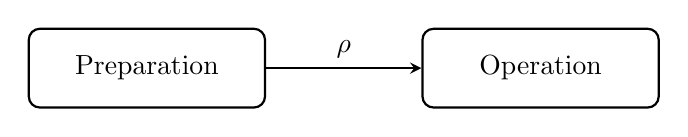
\begin{tikzpicture}[>=stealth,thick]
\node[draw,rounded corners,minimum width=3cm,minimum height=1cm] (a) at (0,0) {Preparation};
\node[draw,rounded corners,minimum width=3cm,minimum height=1cm] (b) at (5,0) {Operation};
\draw[->] (a) -- node[above] {$\rho$} (b);
\end{tikzpicture}
\par\medskip
\begin{minipage}{.55\textwidth}
\raggedright\footnotesize Source: prepared for this example.
\end{minipage}
\end{figure}

  \chapter{Methodology}
The analysis of quantum-information protocols requires the initial state, the allowed operations and the measurement procedure to be specified. Equation~\eqref{eq:qubit} gives a normalized-state example.

The protocol introduced by \textcite{bennett1993} provides a reference for transferring quantum states using classical communication and previously shared entanglement.

  \chapter{Results and discussion}
Table~\ref{tab:estados} lists two representations of quantum states.
\begin{table}[htbp]
\centering\caption{Representations of quantum states.}\label{tab:estados}
\begin{tabularx}{.84\textwidth}{@{}lX@{}}\toprule
State & Representation \\\midrule
Computational & $\lvert0\rangle$ \\
Superposition & $(\lvert0\rangle+\lvert1\rangle)/\sqrt{2}$ \\\bottomrule
\end{tabularx}
\par\medskip
\begin{minipage}{.84\textwidth}
\raggedright\footnotesize Source: prepared for this example.
\end{minipage}
\end{table}
% Replace the example table and this chapter with your research findings.

  \chapter{Conclusions}
% Replace the following line with your research conclusions.
[Insert your conclusions here.]

\else
  \chapter{\TextoIdioma{Introdução}{Introduction}}
\label{cap:introducao}
A informação quântica descreve a preparação, a transformação e a transmissão de estados físicos segundo a mecânica quântica. Os fundamentos matemáticos e computacionais da área são apresentados por \textcite{nielsen2010}.

Na teoria clássica da comunicação, \textcite[p.~379]{shannon1948} apresenta como objetivo \enquote{reproducing at one point either exactly or approximately a message selected at another point.}

A descrição de sistemas quânticos utiliza estados em espaços de Hilbert e operações compatíveis com as regras da teoria. Esses conceitos fornecem a linguagem para a análise de protocolos de processamento de informação.

  \chapter{\TextoIdioma{Fundamentação teórica}{Theoretical background}}
\label{cap:fundamentacao}
\section{\TextoIdioma{Estados e operadores}{States and operators}}
Um qubit puro é representado no espaço de Hilbert bidimensional por
\begin{equation}\label{eq:qubit}
  \lvert\psi\rangle=\alpha\lvert0\rangle+\beta\lvert1\rangle,
  \qquad |\alpha|^{2}+|\beta|^{2}=1.
\end{equation}
Estados gerais são representados por operadores densidade $\rho\succeq0$ com $\operatorname{Tr}\rho=1$. A entropia de von Neumann é
\begin{equation}\label{eq:entropia}
  S(\rho)=-\operatorname{Tr}\bigl(\rho\log_{2}\rho\bigr).
\end{equation}
A interpretação da compressão de informação quântica é discutida em \textcite{schumacher1995}. 

\section{\TextoIdioma{Representação esquemática}{Schematic representation}}
A Figura~\ref{fig:fluxo} apresenta um esquema simplificado de preparação e transformação de um estado.
\begin{figure}[htbp]
\centering
\caption{Esquema de preparação e transformação de um estado.}
\label{fig:fluxo}
\vspace{.35cm}
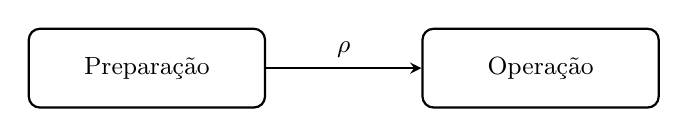
\begin{tikzpicture}[>=stealth,thick, every node/.style={font=\small}]
\node[draw,rounded corners,minimum width=3cm,minimum height=1cm] (a) at (0,0) {Preparação};
\node[draw,rounded corners,minimum width=3cm,minimum height=1cm] (b) at (5,0) {Operação};
\draw[->] (a) -- node[above] {$\rho$} (b);
\end{tikzpicture}
\par\medskip
\begin{minipage}{.55\textwidth}
\raggedright\footnotesize Fonte: elaboração própria.
\end{minipage}
\end{figure}

  \chapter{\TextoIdioma{Metodologia}{Methodology}}
A análise de protocolos de informação quântica exige especificar o estado inicial, as operações empregadas e as medidas efetuadas. A Equação~\eqref{eq:qubit} fornece um exemplo de estado normalizado.

O protocolo apresentado por \textcite{bennett1993} constitui uma referência para a transferência de estados quânticos com o auxílio de comunicação clássica e emaranhamento previamente compartilhado.

  \chapter{\TextoIdioma{Resultados e discussão}{Results and discussion}}
A Tabela~\ref{tab:estados} reúne duas representações de estados quânticos.
\begin{table}[htbp]
\centering
\caption{Representações de estados quânticos.}
\label{tab:estados}
\begin{tabularx}{.84\textwidth}{@{}lX@{}}
\toprule
Estado & Representação \\
\midrule
Computacional & $\lvert0\rangle$ \\
Superposição & $(\lvert0\rangle+\lvert1\rangle)/\sqrt{2}$ \\
\bottomrule
\end{tabularx}
\par\medskip
\begin{minipage}{.84\textwidth}
\raggedright\footnotesize Fonte: elaboração própria.
\end{minipage}
\end{table}

% Substitua a tabela de exemplo e este capítulo pelos resultados de sua pesquisa.

  \chapter{\TextoIdioma{Conclusões}{Conclusions}}
% Substitua esta linha pelas conclusões da sua pesquisa.
[Insira aqui as conclusões.]

\fi

\postextual
\printbibliography[heading=bibintoc,title={\TextoIdioma{REFERÊNCIAS}{REFERENCES}}]
% Para apendices/anexos/glossario, ative apenas o arquivo desejado.
% \chapter*{\TextoIdioma{GLOSSÁRIO}{GLOSSARY}}
\phantomsection\addcontentsline{toc}{chapter}{\TextoIdioma{GLOSSÁRIO}{GLOSSARY}}
\noindent\textbf{Qubit}: \TextoIdioma{sistema quântico efetivo descrito por um espaço de Hilbert de dimensão dois.}{effective quantum system described by a two-dimensional Hilbert space.}

% \begin{apendicesenv}
\partapendices
\ifDocumentoIngles
\chapter{Additional derivations}
\else
\chapter{Desenvolvimento complementar}
\fi
\TextoIdioma{Material produzido pelo autor, a ser preenchido quando necessário.}{Author-produced material, to be completed when necessary.}
\end{apendicesenv}

% \begin{anexosenv}
\partanexos
\ifDocumentoIngles
\chapter{Supplementary document}
\else
\chapter{Documento suplementar}
\fi
\TextoIdioma{Inclua apenas documentos de terceiros com a identificação da fonte e observância de direitos autorais.}{Include third-party documents only when properly credited and used in accordance with copyright rules.}
\end{anexosenv}

\end{document}
